
\renewcommand\thesection{\Roman{section}}
\setcounter{section}{1}
\section{Das direkte Problem}
\renewcommand\thesection{\arabic{section}}
\renewcommand\thesubsection{\arabic{subsection}}
\setcounter{subsection}{2}
\setcounter{section}{3}

In diesem Abschnitt formulieren wir das direkte Problem und zeigen Existenz und Eindeutigkeit von Lösungen.
\paragraph{Annahmen:}\
\begin{enumerate}[label=(\roman*)]
	\item Brechungsindex: \(n^2\in L^\infty(\R^3)\), außerdem existiert ein \(R>0\), sodass \(n^2=1\) fast überall in \(\R^3\setminus B_R(0)\) und \(\RE n^2>0, \;\IM n^2\geq0\) fast überall in \(\R^3\),
	\item Wellenzahl: \(k\in\R,\,k>0\),
	\item Quellterm: \(f\in L^2(\R^3)\), \(f=0\) fast überall in \(\R^3\setminus B_R(0)\),
	\item Primärfeld: \(u^i(x)=\e^{\ii kx\cdot d}\), \(x\in\R^3\), wobei \(d\in\SS^2\).
\end{enumerate}
Das \bol{direkte Problem} besteht darin, anhand der gegebenen Größen \(n^2,k,f\) und \(u^i\) eine Lösung \(u=u^i+u^s\) der Helmholtzgleichung
\begin{equation}
	\label{helmholtzgleichung dp}\tag{3.a}
	\Delta u+k^2n^2u=f\;\;\;\;\te{ in }\R^3,
\end{equation}
zu finden, sodass \(u^s\coloneqq u-u^i\) die \hypertarget{SABdp}{SAB}
\begin{equation}
	\label{SAB direktes problem}\tag{3.b}
	\frac{\p u^s}{\p r}(x)-\ii ku^s(x)=o\Big(\frac{1}{r}\Big),\;\;\;\;\te{ für }r=|x|\rarr\infty,
\end{equation}
gleichmäßig bzgl. \(\widehat{x}=\frac{x}{|x|}\in\SS^2\) erfüllt.
\begin{no counter definition}
	Eine \bol{klassische Lösung} von \eqref{helmholtzgleichung dp}-\eqref{SAB direktes problem} ist ein \(u\in\CC^2(\R^3)\), das \eqref{helmholtzgleichung dp}-\eqref{SAB direktes problem} erfüllt.
\end{no counter definition}
Unter der Annahme, dass \(n^2\in\CC^1(\R^3)\) und \(f\in\CC^1(\R^3)\), kann Existenz und Eindeutigkeit von klassischen Lösungen gezeigt werden. Da wir auch nicht-glatte Brechungsindizes und Quellen zulassen, müssen wir einen allgemeineren Lösungsbegriff betrachten.

\subsection{Sobolevräume und schwache Lösungen}
Bevor wir Sobolevräume einführen, wiederholen wir einige Resultate zur Approximation von \(L^p\)-Funktionen durch glatte Funktionen. In diesem Abschnitt sei \(\Omega\subset\R^N\) offen.
\begin{lem}\label{lem: glm konv von funktionenfolgen auf Lp}
	Sei \(\fn\) eine Folge in \(L^p(\Omega)\), \(1\leq p\leq\infty\), und \(f\in L^p(\Omega)\), sodass \(\|f-f_n\|_p\lorarr0\). Dann gibt es eine Teilfolge \((f_{n_k})_k\) und eine Funktion \(h\in L^p(\Omega)\),sodass
	\begin{enumerate}[label=(\alph*)]
		\item \(f_{n_k}(x)\lorarr f(x)\) fast überall in \(\Omega\),
		\item\label{lemma 3.1 b} \(|f_{n_k}|\leq h\) für alle \(k\in\N\), fast überall in \(\Omega\).
	\end{enumerate}
\end{lem}
\begin{proof}
	Für \(p=\infty\) folgt die Behauptung unmittelbar. Sei also \(1\leq p<\infty\). Da \(\fn\) eine Cauchyfolge in \(L^p(\Omega)\) ist, können wir eine Teilfolge \((f_{n_k})\) auswählen, sodass
	\begin{equation*}
		\|f_{n_{k+1}}-f_{n_k}\|_p\leq\frac{1}{2^k},\;\;\;\;\te{ für alle }k\geq1.
	\end{equation*}
	Sei
	\begin{equation*}
		g_m(x)\coloneqq\sum_{k=1}^m\big|f_{n_{k+1}}(x)-f_{n_k}(x)\big|,
	\end{equation*}
	dann ist \(\|g_m\|_p\leq1\) und mit dem Satz von Levi folgt, dass \(g_m(x)\lorarr g(x)\) fast überall in \(\Omega\) für ein \(g\in L^p(\Omega)\). Andererseits ist für \(\ell> k\geq 2\)
	\begin{equation*}
		\big|f_{n_\ell}(x)-f_{n_k}(x)\big|
		\leq\big|f_{n_\ell}(x)-f_{n_{\ell-1}}(x)\big|+\ldots+\big|f_{n_{k+1}}(x)-f_{n_k}(x)\big|\leq g(x)-g_{k-1}(x),
	\end{equation*}
	und damit \(f_{n_k}\lorarr f^\ast(x)\) fast überall in \(\Omega\). Wegen
	\begin{equation*}
		\big|f^\ast(x)-f_{n_k}(x)\big|\leq g(x),\;\;\;\;\te{ für }k\geq 2,
	\end{equation*}
	ist \(f^\ast\in L^p(\Omega)\) und mit dem Satz von Lebesgue folgt, dass \(f_{n_k}\lorarr f^\ast\) in \(L^p(\Omega)\), also \(f^\ast=f\) fast überall. Zusätzlich ist \(\big|f_{n_k}(x)\big|\leq\big|f^\ast(x)\big|+g(x)\), woraus \ref{lemma 3.1 b} folgt.
\end{proof}
\begin{thm}\label{thm: Cc dicht in Lp}
	Der Raum
	\begin{equation*}
		\Cc(\R^N)=\{f\in\CC(\R^N)\mid f(x)=0\te{ für alle }x\in\R^N\setminus K\te{, wobei }K\te{ kompakt ist}\}
	\end{equation*}
	der stetigen Funktionen mit kompaktem Träger ist dicht in \(L^p(\R^N)\) für \(1\leq p<\infty\).
\end{thm}
\begin{proof}
	Zuerst zeigen wir, dass zu gegebenem \(f\in L^p(\R^N)\) und \(\varepsilon>0\) eine Funktion \(g\in L^\infty(\R^N)\) und \(K\subset\R^N\) kompakt existiert, sodass \(g=0\) in \(\R^N\setminus K\) und
	\begin{equation*}
		\|f-g\|_p<\varepsilon.
	\end{equation*}
	Dazu betrachten wir die Abschneidefunktion \(\func{T_n}{\R}{\R}\),
	\begin{equation*}
		T_n(r)=
		\begin{cases}
			r,&\te{ falls }|r|\leq n,\\
			\frac{nr}{|r|},&\te{ falls }|r|>n.
		\end{cases}
	\end{equation*}
	Wir bezeichnen mit \(\chi_n\) die charakteristische Funktion zu \(B_n(0)\) und definieren \(f_n\coloneqq\chi_n\cdot \big(T_n\circ f\big)\). Nach dem Satz von Lebesgue folgt \(\|f_n-f\|_p\lorarr0\), und wir können \(g=f_n\) mit \(n\) groß genug wählen.
	
	Nach dem Satz von Lusin (Maßtheorie) gibt es für alle \(\delta>0\) eine Funktion \(g_1\in\CC(\R^N)\), sodass
	\begin{equation*}
		\|g-g_1\|_1\leq\delta.
	\end{equation*}
	Wir können annehmen, dass \(\|g_1\|_\infty\leq\|g\|_\infty\) (sonst ersetze \(g_1\) durch \(T_ng_1\) mit \(n=\|g\|_\infty\)). Damit ist
	\begin{equation*}
		\|g-g_1\|_p\leq\|g-g_1\|_1^\frac{1}{p}\|g-g_1\|_\infty^{1-\frac{1}{p}}\leq\delta^{\frac{1}{p}}\big(2\|g\|_\infty\big)^{1-\frac{1}{p}}.
	\end{equation*}
	Wählt man \(\delta\) klein genug, sodass
	\begin{equation*}
		\delta^\frac{1}{p}\big(2\|g\|_\infty\big)^{1-\frac{1}{p}}<\varepsilon,
	\end{equation*}
	dann folgt die Behauptung.
\end{proof}
\begin{de+sa}[Faltung]\label{def und satz: faltung}
	Sei \(f\in L^1(\R^N)\) und \(g\in L^p(\R^N)\) mit \(1\leq p\leq\infty\). Dann ist für f.a. (fast alle) \(x\in\R^N\) die Funktion
	\begin{equation*}
		y\mapsto f(x-y)g(y),
	\end{equation*}
	integrierbar auf \(\R^N\) und wir definieren
	\begin{equation*}
		(f\ast g)(x)\coloneqq\intRN f(x-y)g(y)\dy,\;\;\;\;x\in\R^N.
	\end{equation*}
	Dann ist \(f\ast g\in L^p(\R^N)\) und 
	\begin{equation*}
		\|f\ast g\|_p\leq\|f\|_1\|g\|_p.
	\end{equation*}
\end{de+sa}
\begin{proof}
	Siehe Funktionalanalysis. (weglassen)
\end{proof}
\begin{definition}
	Sei \(\func{f}{\R^N}{\R}\). Betrachte die Familie \((\omega_i)_{i\in I}\) aller offenen Mengen, auf denen \(f\) f.ü. (fast überall) verschwindet. Setze \(\omega\coloneqq\bigcup_{i\in I}\omega_i\), dann ist \(f=0\) f.ü. in \(\omega\). Der \bol{Träger} von \(f\) ist definiert als
	\begin{equation*}
		\support f\coloneqq\R^N\setminus\omega.
	\end{equation*}
\end{definition}
\begin{lem}\label{lem: supp(f*g) subset suppf + supp g}
	Sei \(f\in L^1(\R^N)\) und \(g\in L^p(\R^N)\) mit \(1\leq p\leq\infty\). Dann ist
	\begin{equation*}
		\support(f\ast g)\subset\overline{\support(f)+\support(g)}.
	\end{equation*}
\end{lem}
\begin{proof}
	Übung! (weglassen)
\end{proof}
\begin{definition}
	Sei \(\Omega\subset\R^N\) offen und \(1\leq p<\infty\). Eine Funktion \(\func{f}{\Omega}{\R}\) gehört zu \(\bm{\Lloc^p(\Omega)}\), falls \(\chi_Kf\in L^p(\Omega)\) für jede kompakte Teilmenge \(K\subset\Omega\).
\end{definition}
\paragraph{Beachte:} Falls \(f\in\Lloc^p(\Omega)\), dann ist \(f\in\Lloc^1(\Omega)\).
\begin{satz}
	Sei \(f\in\Cc(\R^N)\) und \(g\in\Lloc^1(\R^N)\). Dann ist \((f\ast g)(x)\) wohldefiniert für alle \(x\in\R^N\) und \(f\ast g\in\CC(\R^N)\).
\end{satz}
\begin{proof}
	Für alle \(x\in\R^N\) ist \(y\mapsto f(x-y)g(y)\) integrierbar auf \(\R^N\) und damit \((f\ast g)(x)\) wohldefiniert. Sei \(\xn\) eine Folge in \(\R^N\) mit \(x_n\rarr x\) und \(K\subset\R^N\) kompakt, sodass
	\begin{equation*}
		\big(x_n-\support(f)\big)\subset K,\;\;\;\;\te{ für alle }n\in\N.
	\end{equation*}
	Dann ist \(f(x_n-y)=0\) für alle \(n\in\N\) und \(y\notin K\). Aus der gleichmäßigen Stetigkeit von \(f\) folgt nun, dass
	\begin{equation*}
		|f(x_n-y)-f(x-y)|\leq\varepsilon_n\chi_K(y),
	\end{equation*}
	für alle \(n\in\N\), \(y\in\R^N\) mit \(\varepsilon_n\rarr0\). Daraus folgt, dass
	\begin{equation*}
		|(f\ast g)(x_n)-(f\ast g)(x)|\leq\varepsilon_n\int_K|g(y)|\dy\lorarr0.
	\end{equation*}
\end{proof}
\begin{definition}[Multiindex]
	Ein \bol{Multiindex} ist ein Vektor \(\alpha=(\alpha_1,\ldots,\alpha_N)\) mit \(\alpha_i\in\N_0\) und
	\begin{equation*}
		|\alpha|=\sum_{i=1}^N\alpha_i,\;\;\;\;
		\alpha!=\prod_{i=1}^{N}\alpha_i!,\;\;\;\;
		x^\alpha=x_1^{\alpha_1}\cdot\ldots\cdot x_N^{\alpha_N},\;\;\;\;
		\D^\alpha u\coloneqq\frac{\p^{|\alpha|}}{\p x_1^{\alpha_1}\ldots\p x_N^{\alpha_N}}u.
	\end{equation*}
\end{definition}
\begin{satz}
	Sei \(f\in\Cc^k(\R^N)\), \(k\geq1\), und \(g\in\Lloc^1(\R^N)\). Dann ist \(f\ast g\in\CC^k(\R^N)\) und
	\begin{equation*}
		\D^\alpha(f\ast g)=(\D^\alpha f)\ast g,\;\;\;\;\;\te{ für alle }\alpha\te{ mit }|\alpha|\leq k.
	\end{equation*}
	Insbesondere ist für \(f\in\Cc^\infty(\R^N)\) und \(g\in\Lloc^1(\R^N)\) auch \(f\ast g\in\CC^\infty(\R^N)\).
\end{satz}
\begin{proof}
	Mit Induktion genügt es, den Fall \(k=1\) zu betrachten. Sei \(x\in\R^N\) und \(h\in\R^N\) mit \(|h|<1\). Dann ist für alle \(y\in\R^N\)
	\begin{align*}
		&\big|f(x+h-y)-f(x-y)-h\cdot\nabla f(x-y)\big|\\
		&=\Big|\int_0^1h\cdot\nabla f(x+sh-y)-h\cdot\nabla f(x-y)\ds\Big|\leq|h|\varepsilon(|h|),
	\end{align*}
	mit \(\varepsilon(|h|)\rarr0\), falls \(|h|\rarr0\), da \(\nabla f\) gleichmäßig stetig auf \(\R^N\) ist. Sei \(K\subset\R^N\) kompakt, sodass \(x+B_1(0)-\support(f)\subset K\). Dann ist für alle \(y\notin K\), \(h\in B_1(0)\)
	\begin{equation*}
		f(x+h-y)-f(x-y)-h\cdot\nabla f(x-y)=0,
	\end{equation*}
	und damit
	\begin{equation*}
		\big|f(x+h-y)-f(x-y)-h\cdot\nabla f(x-y)\big|\leq|h|\varepsilon(|h|)\chi_K(y),
	\end{equation*}
	für alle \(y\in\R^N\), \(h\in B_1(0)\). Für \(h\in B_1(0)\) gilt also
	\begin{equation*}
		\big|(f\ast g)(x+h)-(f\ast g)(x)-h\cdot\big((\nabla f)\ast g\big)(x)\big|
		\leq|h|\varepsilon(|h|)\int_K|g(y)|\dy.
	\end{equation*}
	Daraus folgt, dass \(f\ast g\) stetig differentierbar ist mit \(\nabla(f\ast g)=(\nabla f)\ast g\).
\end{proof}
\begin{definition}
	Eine Folge von \bol{Glättungskernen} (Mollifiern) \((\rho_n)_{n\geq1}\) ist eine Folge von Funktionen auf \(\R^N\), sodass für alle \(n\in\N\)
	\begin{equation*}
		\rho_n\in\Cc^\infty(\R^N),\;\;\;\;
		\support\rho_n\subset\overline{B_{\frac{1}{n}}(0)},\;\;\;\;
		\intRN\rho_n\dx=1,\;\;\;\;
		\rho_n\geq0.
	\end{equation*}
\end{definition}
\begin{bsp}
	Sei
	\begin{equation*}
		\rho(x)=
		\begin{cases}
			\e^{\frac{1}{|x|^2-1}},&\te{ für }|x|<1,\\
			0,&\text{ für }|x|\geq1.
		\end{cases}
	\end{equation*}
	Dann ist durch \(\rho_n(x)=cn^N\rho(nx)\) mit \(c=\big(\intRN \rho(x)\dx\big)^{-1}\) eine Folge von Glättungskernen gegeben.
\end{bsp}
\begin{satz}\label{satz: glm konvergenz von faltung mit mollifier für C}
	Sei \(f\in\CC(\R^N)\). Dann konvergiert \((\rho_n\ast f)\overset{\n\rarr\infty}{\lorarr}f\) gleichmäßig auf kompakten Teilmengen von \(\R^N\).
\end{satz}
\begin{proof}
	Sei \(K\subset\R^N\) kompakt. Zu \(\varepsilon>0\) gibt es \(\delta>0\), sodass
	\begin{equation*}
		|f(x-y)-f(x)|<\varepsilon,\;\;\;\;\te{ für alle }x\in K,y\in B_\delta(0).
	\end{equation*}
	Ferner ist für alle \(x\in\R^N\)
	\begin{align*}
		(\rho_n\ast f)(x)-f(x)&=\intRN\big(f(x-y)-f(x)\big)\rho_n(y)\dy\\
		&=\int_{B_\frac{1}{n}(0)}\big(f(x-y)-f(x)\big)\rho_n(y)\dy.
	\end{align*}
	Für \(n>\frac{1}{\delta}\) und \(x\in K\) erhalten wir, dass
	\begin{equation*}
		|(\rho_n\ast f)(x)-f(x)|\leq\varepsilon\intRN\rho_n(y)\dy=\varepsilon.
	\end{equation*}
\end{proof}
\begin{thm}\label{thm: glm konvergenz von faltung mit mollifier für Lp}
	Sei \(f\in L^p(\R^N)\) mit \(1\leq p<\infty\). Dann konvergiert \((\rho_n\ast f)\overset{n\rarr\infty}{\lorarr}f\) in \(L^p(\R^N)\).
\end{thm}
\begin{proof}
	Sei \(\varepsilon>0\) und \(f_1\in\Cc(\R^N)\), sodass \(\|f-f_1\|_p<\varepsilon\) (siehe Theorem \ref{thm: Cc dicht in Lp}). Nach Satz \ref{satz: glm konvergenz von faltung mit mollifier für C} konvergiert \((\rho_n\ast f_1)\lorarr f\) gleichmäßig auf jeder kompakten Teilmenge von \(\R^N\). Andererseits ist nach Lemma \ref{lem: supp(f*g) subset suppf + supp g}
	\begin{equation*}
		\support(\rho_n\ast f_1)\subset\overline{B_{\frac{1}{n}}(0)}+\support(f_1)\subset\overline{B_1(0)}+\support(f_1),
	\end{equation*}
	wobei \(\overline{B_1(0)}+\support(f_1)\) eine kompakte Menge ist. Damit konvergiert
	\begin{equation*}
		\|(\rho_n\ast f_1)-f_1\|_p\overset{n\rarr\infty}{\lorarr}0.
	\end{equation*}
	Nun schreiben wir
	\begin{align*}
		(\rho_n\ast f)-f&=\big(\rho_n\ast(f-f_1)\big)+\big((\rho_n\ast f_1)-f_1\big)+f_1-f\\
		&\leq\underbrace{\|\rho_n\|_1}_{=1}\|f-f_1\|_p+\big((\rho_n\ast f_1)-f_1\big)+f_1-f.
	\end{align*}
	Mit Satz \ref{def und satz: faltung} folgt
	\begin{equation*}
		\|(\rho_n\ast f)-f\|_p\leq2\|f_1-f\|_p+\|(\rho_n\ast f_1)-f_1\|_p,
	\end{equation*}
	also
	\begin{equation*}
		\limsupn\|(\rho_n\ast f)-f\|_p\leq2\varepsilon,\;\;\;\;\te{ für alle }\varepsilon>0.
	\end{equation*}
	Da \(\varepsilon>0\) beliebig klein gewählt werden kann, gilt
	\begin{equation*}
		\limn\|(\rho_n\ast f)-f\|_p=0.
	\end{equation*}
\end{proof}
\begin{cor}\label{kor: int uf = 0 für u in L1loc, also u = 0 fü}
	Sei \(\Omega\subset\R^N\) offen und \(u\in\Lloc^1(\Omega)\), sodass
	\begin{equation*}
		\int_\Omega uf\dx=0,
	\end{equation*}
	 für alle \(f\in\Cc^\infty(\Omega)=\{\phi\in\CC^\infty(\Omega)\mid\phi=0\te{ in }\Omega\setminus K\te{ für ein }K\subset\Omega\te{ kompakt}\}\). Dann ist \(u=0\) f.ü. in \(\Omega\).
\end{cor}
\begin{proof}
	Sei \(g\in L^\infty(\R^N)\) mit kompaktem Träger \(\support g\subset\Omega\), also insb. auch \(g\in L^1(\R^N)\). Wir setzen \(g_n\coloneqq\rho_n\ast g\), dann ist \(g_n\in\Cc^\infty(\Omega)\) für \(n\) groß genug. Daher ist
	\begin{equation}
		\label{integral ugn = 0 für n groß}
		\int_\Omega ug_n\dx=0,\;\;\;\;\;\te{ für }n\te{ groß genug.}
	\end{equation}
	Da \(g_n\lorarr g\) in \(L^1(\R^N)\) nach Theorem \ref{thm: glm konvergenz von faltung mit mollifier für Lp}, gibt es eine Teilfolge, hier mit \(g_{n_k}\) bezeichnet, sodass \(g_{n_k}\lorarr g\) f.ü. auf \(\Omega\) nach Lemma \ref{lem: glm konv von funktionenfolgen auf Lp}. Außerdem ist nach Young
	\begin{equation*}
		\|g_{n_k}\|_{L^\infty(\Omega)}\leq\underbrace{\|\rho_{n_k}\|_{L^1(\R^N)}}_{=1}\|g\|_{L^\infty(\Omega)}.
	\end{equation*}
	Für \(k\rarr\infty\) folgt aus \eqref{integral ugn = 0 für n groß} mit dem Satz von Lebesgue, dass
	\begin{equation}
		\label{integral ug = 0}
		\intRN ug\dx=\int_\Omega ug\dx=0.
	\end{equation}
	Sei nun \(K\subset\Omega\) kompakt und wähle
	\begin{equation*}
		g=
		\begin{cases}
			\sign u,&\te{ in }K,\\
			0,&\te{ in }\R^N\setminus K.
		\end{cases}
	\end{equation*}
	Dann folgt mit \eqref{integral ug = 0}, dass \(\int_K|u|\dx=0\), also \(u=0\) f.ü. in \(K\). Da \(K\subset\Omega\) beliebig war, folgt \(u=0\) f.ü. in \(\Omega\).
\end{proof}
\begin{cor}\label{kor: Ccinfty dicht in Lp}
	Sei \(\Omega\subset\R^N\) offen. Dann ist \(\Cc^\infty(\Omega)\subset L^p(\Omega)\) dicht für \(1\leq p<\infty\).
\end{cor}
\begin{proof}
	Sei \(f\in L^p(\Omega)\). Wir setzen
	\begin{equation*}
		\overline{f}(x)=
		\begin{cases}
			f(x),&\te{ für }x\in\Omega,\\
			0,&\te{ für }x\in\R^N\setminus\overline{\Omega},
		\end{cases}
	\end{equation*}
	es gilt \(\overline{f}\in L^p(\R^N)\). Sei \((K_n)_n\) eine Folge von kompakten Teilmengen des \(\R^N\), sodass \(\bigcup_{n=1}^\infty K_n=\Omega\) und \(\dist(K_n,\Omega^\cc)\geq\frac{2}{n}\) für alle \(n\).\vspace{4cm}
	
	
	\noindent Beispielsweise
	\begin{equation*}
		K_n=\big\{x\in\Omega\mid|x|\leq n\te{ und }\dist(x,\Omega^\cc)\geq\frac{2}{n}\big\},
	\end{equation*}
	Setze \(g_n\coloneqq\chi_{K_n}\overline{f}\) und \(f_n\coloneqq\rho_n\ast g_n\), sodass
	\begin{equation*}
		\support(f_n)\subset\overline{B_\frac{1}{n}(0)}+K_n\subset\Omega.
	\end{equation*}
	Es folgt, dass \(f_n\in\Cc^\infty(\Omega)\). Andererseits gilt
	\begin{align*}
		\|f-f_n\|_{L^p(\Omega)}&=\|\overline{f}-f_n\|_{L^p(\Omega)}\\
		&\leq\|(\rho_n\ast g_n)-(\rho_n\ast\overline{f})\|_{L^p(\R^N)}+\|(\rho_n\ast\overline{f})-\overline{f}\|_{L^p(\Omega)}\\
		\te{\scriptsize Young}&\leq\underbrace{\|\rho_n\|_{L^1(\Omega)}}_{=1}\|g_n-\overline{f}\|_{L^p(\R^N)}+\|(\rho_n\ast\overline{f})-\overline{f}\|_{L^p(\Omega)}.
	\end{align*}
	Nach dem Satz von Lebesgue und Theorem \ref{thm: glm konvergenz von faltung mit mollifier für Lp}
	\begin{equation*}
		\|g_n-\overline{f}\|_{L^p(\R^N)}\overset{n\rarr\infty}{\lorarr}0,\;\;\;\te{ und } \;\;\;\|(\rho_n\ast\overline{f})-\overline{f}\|_{L^p(\Omega)}\overset{n\rarr\infty}{\lorarr}0,
	\end{equation*}
	also
	\begin{equation*}
		\|f-f_n\|_{L^p(\Omega)}\overset{n\rarr\infty}{\lorarr}0,\;\;\;\;\te{ für }n\rarr\infty.
	\end{equation*}
\end{proof}

\subsubsection*{Schwache Ableitungen}
Sei \(\Omega\subset\R^N\) offen und \(u\in\CC^{|\alpha|}(\Omega)\), dann ist
\begin{equation}
	\label{herleitung schwache ableitung}
	\int_\Omega u\D^\alpha\phi\dx=(-1)^{|\alpha|}\int_\Omega(\D^\alpha u)\phi\dx,\;\;\;\;\te{ für alle }\phi\in\Cc^\infty(\Omega).
\end{equation}
(partielle Integration)
\begin{definition}\label{def: schwache ableitung}
	Eine Funktion \(u\in\Lloc^1(\Omega)\) besitzt eine \(\bm{\alpha}\)\bol{-te schwache Ableitung} in \(\Omega\), wenn es ein \(v\in\Lloc^1(\Omega)\) gibt, sodass
	\begin{equation*}
%		\label{definition schwache ableitung}
		\int_\Omega u\D^\alpha\phi\dx=(-1)^{|\alpha|}\int_\Omega v\phi\dx,\;\;\;\;\te{ für alle }\phi\in\Cc^\infty(\Omega).
	\end{equation*}
\end{definition}
\begin{lem}\label{lem: eindeutigkeit der schwachen ableitung}
	Die schwache Ableitung ist eindeutig, falls sie existiert. Wenn eine Funktion klassisch differentierbar ist, so ist sie auch schwach differentierbar und beide Ableitungen stimmen überein.
\end{lem}
\begin{proof}
	Wenn \(v\) und \(w\) schwache Ableitungen von \(u\) sind, so ist
	\begin{equation*}
		\int_\Omega u\D^\alpha\phi\dx=(-1)^{|\alpha|}\int_\Omega v\phi\dx=(-1)^{|\alpha|}\int_\Omega w\phi\dx,\;\;\;\;\te{ für alle }\phi\in\Cc^\infty(\Omega).
	\end{equation*}
	Also gilt für alle \(\phi\in\Cc^\infty(\Omega)\)
	\begin{equation*}
		\int_\Omega v\phi\dx=\int_\Omega w\phi\dx.
	\end{equation*}
	Korollar \ref{kor: int uf = 0 für u in L1loc, also u = 0 fü} liefert \(v=w\) f.ü. in \(\Omega\). Die zweite Behauptung folgt aus \eqref{herleitung schwache ableitung}.
\end{proof}
\begin{bsp}
	Betrachte \(N=1\), \(\Omega=(-1,1)\), \(u(x)=|x|\), dann gilt für alle \(\phi\in\Cc^\infty(\Omega)\)
	\begin{align*}
		\int_{-1}^1u(x)\phi'(x)\dx&=-\int_{-1}^0x\phi'(x)\dx+\int_0^1x\phi'(x)\dx\\
		&=\int_{-1}^0\phi(x)\dx-\underbrace{\big[x\phi(x)\big]_{x=-1}^0}_{=0}-\int_0^1\phi(x)\dx+\underbrace{\big[x\phi(x)\big]_{x=0}^1}_{=0}\\
		&=-\int_{-1}^1\sign(x)\phi(x)\dx,
	\end{align*}
	also ist \(\sign\) die schwache Ableitung von \(u\). Um zu überprüfen, ob \(\sign\) schwach differentierbar ist, betrachten wir für beliebiges \(\phi\in\Cc^\infty(\Omega)\)
	\begin{align*}
		\int_{-1}^1\sign(x)\phi'(x)\dx
		&=-\int_{-1}^0\phi'(x)\dx+\int_0^1\phi'(x)\dx\\
		&=-[\phi(x)]_{x=-1}^0+[\phi(x)]_{x=0}^1\\
		&=-2\phi(0).
	\end{align*}
	Es gibt aber kein \(v\in\Lloc^1(\Omega)\) mit \(\int_{-1}^1v(x)\phi(x)\dx=-2\phi(0)\) für alle \(\phi\in\Cc^\infty(\Omega)\) (verwende bspw. Theorem \ref{thm: glm konvergenz von faltung mit mollifier für Lp}). Also ist \(\sign\) nicht schwach differentierbar
\end{bsp}
\begin{bsp}
	Sei \(N=3\), \(\Omega=B_1(0)\) und \(u_\alpha(x)=|x|^{\alpha}\), \(\alpha\in\R\). In Kugelkoordinaten folgt
	\begin{equation*}
		\int_{B_1(0)}u_\alpha(x)\dx=4\pi\int_0^1r^{\alpha+2}\dr,
	\end{equation*}
	also \(u_\alpha\in L^1\big(B_1(0)\big)\) für \(\alpha>-3\). Wegen Lemma \ref{lem: eindeutigkeit der schwachen ableitung} ist \(u_\alpha\) schwach differentierbar in \(B_1(0)\setminus\{0\}\) mit
	\begin{equation*}
		\nabla u_\alpha(x)=\alpha|x|^{\alpha-2}x.
	\end{equation*}
	Partielle Integration liefert für alle \(\phi\in\Cc^\infty\big(B_1(0)\big)\) mit \eqref{greenscher satz 1} für \(u=u_\alpha(\phi e_j)\)
	\begin{equation*}
		\int_{B_1(0)\setminus\overline{B_{\varepsilon}(0)}}u_\alpha(x)\nabla\phi(x)\dx
		=-\int_{B_1(0)\setminus\overline{B_{\varepsilon}(0)}}\phi(x) u_\alpha(x)\dx+\int_{\p B_\varepsilon(0)}\normal(s)u_\alpha(s)\phi(s)\ds(x).
	\end{equation*}
	Für \(\alpha>-2\) sind \(|u_\alpha\nabla\phi|\) und \(|(\nabla u_\alpha)\phi|\) integrierbare Majoranten für die Volumenintegrale, und wir können mit dem Satz von Lebesgue den Grenzübergang \(\varepsilon\rarr0\) durchführen. Außerdem ist
	\begin{equation*}
		\Big|\int_{\p B_\varepsilon(0)}\normal(s)u_\alpha(s)\phi(s)\ds(x)\Big|
		\leq\|\phi\|_\infty\int_{\p B_\varepsilon(0)}\varepsilon^\alpha\ds(x)
		=\|\phi\|_\infty4\pi\varepsilon^{\alpha+2}
		\lorarr0,\;\;\;\;\te{ für }\varepsilon\rarr0.
	\end{equation*}
	Also ist \(u_\alpha\) schwach differentierbar für \(\alpha>-2\).
\end{bsp}

\subsubsection*{Sobolevräume}
Sei \(\Omega\subset\R^N\) offen.
\begin{definition}
	Für \(m\in\N\) sei der \bol{Sobolevraum \(\bm{\H^m(\Omega)}\)} definiert durch
	\begin{align*}
		\H^m(\Omega)\coloneqq\big\{u\in L^2(\Omega)\mid&\,\forall\alpha\in\N_0^N,|\alpha|\leq m\,\exists v_\alpha\in L^2(\Omega)\,\forall\phi\in\Cc^\infty(\Omega)\colon\\
		&\;\;\int_\Omega u\D^\alpha\phi\dx=(-1)^{|\alpha|}\int_\Omega v_\alpha\phi\dx\big\}.
	\end{align*}
	Ersetzt man \(L^2(\Omega)\) durch \(L^p(\Omega)\), \(1\leq p\leq\infty\), so erhält man \(\W^{m,p}(\Omega)\), d.h. \(\H^m(\Omega)=\W^{m,2}(\Omega)\).
\end{definition}
\begin{satz}
	\(\H^m(\Omega)\) ist ein Hilbertraum mit dem Skalarprodukt
	\begin{equation*}
		\scalmo{u}{v}\coloneqq\sum_{|\alpha|\leq m}\scaltwoo{\D^\alpha u}{\D^\alpha v}.
	\end{equation*}
\end{satz}
\begin{proof}
	Die Skalarprodukteigenschaften übertragen sich unmittelbar vom \(L^2\)-Skalarprodukt auf \(L^2(\Omega)\). Um Vollständigkeit zu zeigen sei \((u_k)_k\subset\H^m(\Omega)\) eine Cauchyfolge. Dann ist für alle \(|\alpha|\leq m\) auch \((\D^\alpha u_k)_k\subset L^2(\Omega)\) eine Cauchyfolge mit Grenzwert \(v_\alpha\in L^2(\Omega)\). Sei \(\phi\in\Cc^\infty(\Omega)\), dann ist
	\begin{figure}[!h]
		\centering
		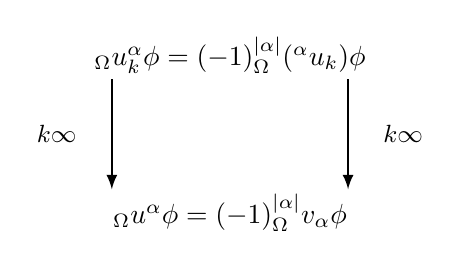
\begin{tikzpicture}
			\node at (0,1){\(\bigintsss_\Omega u_k\D^\alpha\phi\dx=(-1)^{|\alpha|}\bigintsss_\Omega(\D^\alpha u_k)\phi\dx\)};
			
			\node at (0,-1){\(\bigintsss_\Omega u\D^\alpha\phi\dx=(-1)^{|\alpha|}\bigintsss_\Omega v_\alpha \phi\dx\)};
			
			
			\draw[thick,-{latex[scale=3.0]}] (-1.5, 0.7)--(-1.5,-0.7);
			\draw[thick,-{latex[scale=3.0]}] (1.5,0.7)--(1.5,-0.7);
			
			\node at (-2.2,0){\small \(k\rarr\infty\)};
			\node at (2.2,0){\small \(k\rarr\infty\)};
		\end{tikzpicture}
	\end{figure}\\
	d.h. \(u\in\H^m(\Omega)\), \(\D^\alpha u=v_\alpha\), (wobei \(u_k\lorarr u\) in \(L^2(\Omega)\)) und damit \(u_k\lorarr u\) in \(\H^m(\Omega)\).
\end{proof}
\begin{definition}
	Sei \(\Omega\subset\R^N\) offen.
	\begin{align*}
		\Hloc^m(\Omega)&\coloneqq\big\{\func{u}{\Omega}{\C}\mid\chi_{\Omega\cap B_R(0)}u\in\H^m\big(\Omega\cap B_R(0)\big)\te{ für alle }R>0\te{. sodass }\Omega\cap B_R(0)\neq\emptyset\big\}\\
		&=\big\{u \in \Lloc^1(\Omega)\mid u\restrict{\Omega\cap B_R(0)}\in\H^m\big(\Omega\cap B_R(0)\big)\te{ für alle }R>0\te{. sodass }\Omega\cap B_R(0)\neq\emptyset\big\}.
	\end{align*}
\end{definition}
\begin{lem}\label{lem: abschneidefunktionen}
	Sei \(K\subset\Omega\) kompakt. Dann gibt es eine Abschneidefunktion bzgl. \(\{K,\Omega\}\), d.h. eine reellwertige Funktion \(\tau\in\Cc^\infty(\Omega)\) mit \(0\leq\tau\leq1\) und \(\tau=1\) in \(K\). Wenn \(\dist(\p K,\p\Omega)=\delta\), so kann \(\tau\) so gewählt werden, dass
	\begin{equation*}
		|\D^\alpha\tau|\leq C\delta^{-|\alpha|},
	\end{equation*}
	wobei die Konstante \(C\) von \(\alpha\) und \(N\), aber nicht von \(\Omega\) und \(K\) abhängt.
\end{lem}
\begin{proof}
	Da \(K\) kompakt ist, folgt \(\delta>0\). Ferner ist
	\begin{equation*}
		\widetilde{K}\coloneqq\overline{\bigcup_{x\in K}B_\frac{\delta}{2}(x)},
	\end{equation*}
	kompakt und \(\dist(\p\widetilde{K},\p\Omega)=\dist(\p\widetilde{K},\p K)=\frac{\delta}{2}\).\vspace{2.5cm}
	
	
	Setze \(n=\big\lceil\frac{4}{\delta}\big\rceil\), dann ist \(\tau\coloneqq\rho_n\ast\chi_{\widetilde{K}}\) die gesuchte Abschneidefunktion: Da \(|(\D^\alpha\rho_n)(x)|\leq C(\alpha)\delta^{-N-|\alpha|}\), folgt
	\begin{align*}
		|(\D^\alpha\tau)(x)|&
		\leq\int_{B_\frac{1}{n}(x)}\underbrace{|\D^\alpha\rho_n(x-y)|}_{\leq C(\alpha)\delta^{-N-|\alpha|}}\chi_{\widetilde{K}}(y)\dy\\
		&\leq C(\alpha)\delta^{-N-|\alpha|}\underbrace{|B_\frac{1}{n}(x)|}_{\sim(\delta/4)^N}\\
		&\leq C(\alpha,N)\delta^{-|\alpha|}.
	\end{align*}
\end{proof}
\begin{lem}[Zerlegung der Eins]\label{lem: zerlegung der eins}
	Sei \(\{\Omega_\ell\}_{\ell=1,\ldots,L}\) eine offene Überdeckung einer kompakten Menge \(K\subset\R^N\). Dann gibt es (reellwertige) Funktionen \(\psi_\ell\), \(\ell=1,\ldots,L\), sodass
	\begin{equation*}
		\psi_\ell\in\Cc^\infty(\Omega_\ell),\;\;\;\;0\leq\psi_\ell\leq1,\;\;\;\;\sum_{\ell=1}^L\psi_\ell=1,\;\;\;\;\te{ in }K.
	\end{equation*}
\end{lem}
\begin{proof}
	Für alle \(x\in\Omega_\ell\) existiert ein \(r=r(x,\ell)>0\), sodass \(\overline{B_r(x)}\subset\Omega_\ell\), \(x\in\Omega_\ell\), \(\ell=1,\ldots,L\). Die Mengen \(B_{x,\ell}\coloneqq B_r(x)\) bilden eine offene Überdeckung der kompakten Menge \(K\), also existiert eine endliche Überdeckung.
	
	Seien \(B_1^\ell,\ldots,B_{n_\ell}^\ell\) die Bälle mit Index \(\ell=1,\ldots,L\) in dieser Teilüberdeckung, dann ist
	\begin{equation*}
		K_\ell\coloneqq\overline{\bigcup_{i=1}^{n_\ell}B_i^{\ell}}\subset\Omega_\ell,
	\end{equation*}
	kompakt. Sei \(\tau_\ell\) eine Abschneidefunktion bzgl. \(\{K_\ell,\Omega_\ell\}\) wie in Lemma \ref{lem: abschneidefunktionen}, dann gilt
	\begin{equation*}
		0\leq\tau_\ell\leq1,\;\;\;\psi\coloneqq\sum_{\ell=1}^L\tau_\ell\geq1\;\;\te{ in }K\;\;\te{ und }\;\;K\subset\Omega\coloneqq\bigcup_{\ell=1}^L\support(\tau_\ell).
	\end{equation*}
	Es gibt eine offene Menge \(\Omega_0\) mit \(K\subset\Omega_0\) und \(\overline{\Omega}_0\subset\Omega\). Für eine Abschneidefunktion \(\tau_0\) bzgl. \(\{K,\Omega_0\}\) setze
	\begin{equation*}
		\psi_k(x)\coloneqq
		\begin{cases}
			\cfrac{\tau_k(x)\tau_0(x)}{\psi(x)},&\te{ für }x\in\Omega_0,\\
			0,&\te{ sonst.}
		\end{cases}
	\end{equation*}
	Dann sind \(\psi_1,\ldots,\psi_L\) die gesuchte Zerlegung der Eins.
\end{proof}
\begin{lem}[Produktregel]\label{lem: produktregel}
	Sei \(\psi\in\Cc^\infty(\Omega)\) und \(u\in\H^m(\Omega)\), dann ist \(\psi u\in\H^m(\Omega)\) und 
	\begin{equation*}
		\D^\alpha(\psi u)=\sum_{\beta\leq\alpha}\begin{pmatrix}\alpha\\\beta\end{pmatrix}(\D^\beta\psi)(\D^{\alpha-\beta}u),\;\;\;\;\;\;\;\;\;\;\te{ für }|\alpha|\leq m,
	\end{equation*}
	wobei
	\begin{equation*}
		\begin{pmatrix}\alpha\\\beta\end{pmatrix}\coloneqq\prod_{i=1}^N\begin{pmatrix}\alpha_i\\\beta_i\end{pmatrix},
	\end{equation*}
	und \(\beta\leq\alpha\) genau dann, wenn \(\beta_i\leq\alpha_i\) für alle \(i=1,\ldots,N\).
\end{lem}
\begin{proof}
	Mit Induktion reicht es, den Fall \(|\alpha|=1\) zu betrachten. Sei also \(D^\alpha=\frac{\p}{\p x_i}\), dann ist für alle \(\phi\in\Cc^\infty(\Omega)\)
	\begin{align*}
		\int_\Omega\psi u\frac{\p\phi}{\p x_i}\dx
		&=\int_\Omega u\Big(\frac{\p}{\p x_i}(\psi\phi)-\phi\frac{\p}{\p x_i}\psi\Big)\dx\\
		&=-\int_\Omega\Big(\psi\frac{\p u}{\p x_i}+u\frac{\p\psi}{\p x_i}\Big)\phi\dx.
	\end{align*}
	Damit folgt
	\begin{equation*}
		\frac{\p(\psi u)}{\p x_i}=\psi\frac{\p u}{\p x_i}+u\frac{\p \psi}{\p x_i},
	\end{equation*}
	und da \(\psi\) und \(\frac{\p\psi}{\p x_i}\) beschränkt sind, ist \(\psi u\in\H^1(\Omega)\).
\end{proof}
\begin{lem}\label{lem: ableitung in faltung reinziehen für mollifier}
	Sei \(u\in\H^m(\Omega)\) und \(\Omega_0\ssubset\Omega\) offen, d.h. \(\overline{\Omega}_0\) kompakt und \(\overline{\Omega}_0\subset\Omega\). Dann gilt
	\begin{equation*}
		\D^\alpha(\rho_n\ast u)=\rho_n\ast\D^\alpha u,\;\;\;\;\;\;\;\;\;\;\te{ für }|\alpha|\leq m,
	\end{equation*}
	insbesondere \(\rho_n\ast u\lorarr u\) in \(\H^m(\Omega_0)\).
\end{lem}
\begin{proof}
	Sei \(\frac{2}{n}<\dist(\p\Omega_0,\p\Omega)\). Dann ist für \(|\alpha|\leq m\)
	\begin{align*}
		\int_\Omega(\rho_n\ast u)\D^\alpha\psi\dx
		&=\int_\Omega\int_\Omega\rho_n(x-y)u(y)\D^\alpha\psi(x)\dy\dx\\
		&=\int_\Omega\int_\Omega\rho_n(z)u(x-z)\D^\alpha\psi(x)\dx\dz\\
		&=(-1)^{|\alpha|}\int_\Omega\int_\Omega\rho_n(z)\psi(x)\D^\alpha u(x-z)\dx\dz\\
		&=(-1)^{|\alpha|}\int_\Omega(\rho_n\ast\D^\alpha u)\psi\dx,
	\end{align*}
	für alle \(\psi\in\Cc^\infty(\Omega_0)\). Also gilt
	\begin{equation*}
		\D^\alpha(\rho_n\ast u)=\rho_n\ast\D^\alpha u,\;\;\;\;\;\,\te{ für }|\alpha|\leq m.
	\end{equation*}
	Da außerdem \(\D^\alpha u\in L^2(\Omega)\), liefert Theorem \ref{thm: glm konvergenz von faltung mit mollifier für Lp}, dass
	\begin{equation*}
		\D^\alpha(\rho_n\ast u)=\rho_n\ast\D^\alpha u\lorarr\D^\alpha u,\;\;\;\;\;\;\te{ in }L^2(\Omega_0),
	\end{equation*}
	d.h. \(\rho_n\ast u\lorarr u\) in \(\H^m(\Omega_0)\).
\end{proof}
\begin{thm}[Meyers and Serrin]\label{thm: meyers and serrin}
	\(\CC^\infty(\Omega)\cap\H^m(\Omega)\) ist dicht in \(\H^m(\Omega)\).
\end{thm}
\begin{proof}
	\vspace{2cm}
	
	Für \(n\in\N\) sei 
	\begin{equation*}
		\Omega_n=\big\{x\in\Omega\mid\dist(x,\p\Omega)>\frac{2}{n}\te{ und }|x|<n\big\},
	\end{equation*}
	offen und beschränkt. Es gilt \(\Omega=\bigcup_{n\in\N}\Omega_n\) und wir setzen
	\begin{equation*}
		U_n\coloneqq\Omega_{n+1}\cap\big(\R^N\setminus\overline{\Omega}_{n-1}\big),\;\;\qquad\Omega_0=\Omega_{-1}=\emptyset.
	\end{equation*}
	Dazu konstruieren wir wie im Beweis von Lemma \ref{lem: zerlegung der eins} Abschneidefunktionen \(\psi_n\in\Cc^\infty(U_n)\) mit \(\psi_n\geq0\) und \(\sum_{n=1}^\infty\psi_n=1\) in \(\Omega\).
	
	Sei \(u\in\H^m(\Omega)\), dann haben die Funktionen \(\psi_nu\) kompakten Träger in \(\Omega\) und aus Lemma \ref{lem: produktregel} folgt, dass \(\psi_nu\in\H^m(\Omega)\). Zu beliebigem \(\varepsilon>0\) wähle \(\ell_n\in\N\) groß genug, sodass
	\begin{equation*}
		\support\big(\rho_{\ell_n}\ast(\psi_nu)\big)\subset U_n,
	\end{equation*}
	und (mit Lemma \ref{lem: ableitung in faltung reinziehen für mollifier})
	\begin{equation*}
		\|\rho_{\ell_n}\ast(\psi_nu)-\psi_nu\|_{\H^m(\Omega)}<2^{-n}\varepsilon.
	\end{equation*}
	Die Funktion
	\begin{equation*}
		\phi(x)\coloneqq\sum_{n=1}^\infty\big(\rho_{\ell_n}\ast(\psi_nu)\big)(x),
	\end{equation*}
	ist wohldefiniert, da für jedes \(x\in\Omega\) nur endlich viele Terme in der Summe \rec{nicht} verschwinden. Also ist \(\phi\in\CC^\infty(\Omega)\) und in \(\Omega_n\) gilt
	\begin{equation*}
		u=\sum_{i=1}^{n+2}\psi_iu,\qquad\phi=\sum_{i=1}^{n+2}\rho_{\ell_i}\ast(\psi_iu),\qquad\|u-\phi\|_{\H^m(\Omega_n)}\leq\sum_{i=1}^{n+2}\|\psi_iu-\rho_{\ell_i}\ast(\psi_iu)\|_{\H^m(\Omega)}<\varepsilon,
	\end{equation*}
	wobei wir in der letzten Ungleichung ausgenutzt haben, dass \(\|\psi_iu-\rho_{\ell_i}\ast(\psi_iu)\|_{\H^m(\Omega)}\leq2^{-i}\varepsilon\) gilt. Wenden wir den Satz von Levi auf \(|\D^\alpha(u-\phi)|^2\chi_{\Omega_n}\) an, so folgt \(\|u-\phi\|_{\H^m(\Omega)}\leq\varepsilon\).
\end{proof}
\begin{bem}
	Man kann nicht vorgehen wie im Beweis von Korollar \ref{kor: Ccinfty dicht in Lp}: Betrachte \(N=m=1\), \(\Omega=(0,1)\), \(u=1\) in \(\Omega\). Setzen wir \(u\) durch \(0\) zu \(\widetilde{u}\) auf \(\R\) fort und betrachten \(u_n=\delta_n\ast\widetilde{u}\), dann verhält sich \(u_n'\) in den Intervallen \(\big[-\frac{1}{2n},\frac{1}{2n}\big]\) und \(\big[1-\frac{1}{2n},1+\frac{1}{2n}\big]\) wie \(n\). Damit gilt
	\begin{equation*}
		\int_0^1|u_n'|^2\dx\geq Cn>0,
	\end{equation*}
	für alle \(n\in\N\) und \(u_n'\) konvergiert nicht gegen \(u'=0\) in \(L^2(\Omega)\).
\end{bem}
\subsubsection*{Schwache Lösungen}
\begin{definition}\label{def: schwache lösung}
	Eine \bol{schwache Lösung} von \eqref{helmholtzgleichung dp} ist eine Funktion \(u\in\Hloc^1(\R^3)\), sodass 
	\begin{equation}
		\label{schwache lösung definition}
		\int_{\R^3}\nabla u\cdot\nabla\psi-k^2n^2u\psi\dx=-\int_{\R^3}f\psi\dx,\;\;\;\;\;\te{ für alle }\psi\in\Hc^1(\R^3),
	\end{equation}
	wobei
	\begin{equation*}
		\Hc^1(\R^3)\coloneqq\{\phi\in\H^1(\R^3)\mid\support\phi\te{ ist kompakt}\}.
	\end{equation*}
\end{definition}
\begin{counter bem}
	Sei \(u\in\CC^2(\R^3)\) eine klassische Lösung von \(\Delta u+k^2n^2u=f\) in \(\R^3\), dann ist \(u\in\Hloc^1(\R^3)\) und \eqref{schwache lösung definition} ist für alle \(\psi\in\Cc^\infty(\R^3)\) erfüllt (Greensche Formel \eqref{greenscher satz 2}). Da \(\Cc^\infty(\R^3)\subset\Hc^1(\R^3)\) dicht ist (Theorem \ref{thm: meyers and serrin}), gilt \eqref{schwache lösung definition} auch für alle \(\psi\in\Hc^1(\R^3)\). Daher ist jede klassische Lösung von \eqref{helmholtzgleichung dp} auch eine schwache Lösung.
\end{counter bem}
\begin{thm}[(elliptische) Regularität]\label{thm: regularität}
	Sei \(u\in\H^1(\Omega)\) eine schwache Lösung von \(\Delta u+k^2u=0\) in \(\Omega\subset\R^3\) offen, d.h.
	\begin{equation*}
		\int_\Omega\nabla u\cdot\nabla\psi-k^2u\psi\dx=0,\;\qquad\te{ für alle }\psi\in\Hc^1(\Omega),
	\end{equation*}
	dann ist \(u\in\CC^\infty(\Omega)\).
\end{thm}
\begin{proof}
	Gilbarg-Trudinger, Kapitel 7-8.
\end{proof}
Da wir annehmen, dass ein \(R>0\) existiert, sodass
\begin{equation*}
	\Delta u+k^2u=0,\;\qquad\te{ in }\R^3\setminus\overline{B_R(0)},
\end{equation*}
folgt, dass \(u\) und damit auch \(u^s=u-u^i\) in \(\R^3\setminus\overline{B_R(0)}\) glatt ist. Insbesondere macht die \SABdp auch für schwache Lösungen von \eqref{helmholtzgleichung dp} Sinn. Eine schwache Lösung von \eqref{helmholtzgleichung dp}-\eqref{SAB direktes problem} ist also ein \(u\in\Hloc^1(\R^3)\), sodass \eqref{schwache lösung definition} und \eqref{SAB direktes problem} erfüllt sind.

























